\title{Pendolo invertito su rotaia}
\maketitle
\label{sec:pic}


\section{Introduzione}
\paragraph{Il pendolo invertito su rotaia è un sistema facile da modellare,}
ma presenta alcune caratterische che rendono interessante studiarne la controllabilità.
Il sistema è mostrato in figura \ref{fig:pic} e consiste in un pendolo rigido, libero di ruotare e vincolato a muoversi lungo una rotaia rettilinea tramite un carrello. L'unico modo in cui i sistema può interagire con l'esterno è tramite una forza applicata sul carrello lungo la direzione della rotaia. Quando il pendolo è fermo ed è diretto verso l'alto, si trova in un punti di equilibrio instabile e ogni minima perturbazione tenderà a farlo ricadere verso il basso. L'obiettivo che mi pongo è duplice:

\begin{enumerate}
    \item Stabilizzare il pendolo attorno al punto di equilibrio instabile, in modo che sia resistente alle perturbazioni.
    \item Trovare una strategia per portare il pendolo in prossimità del punto di equilibrio instabile, partendo dalla configurazione stabile (\emph{swing-up}).
\end{enumerate}

%todo traduci in italiano
\paragraph{Il sistema è non-lineare e underactuated.} Questo significa che per portare a termine i due obiettivi discussi sopra, è necessario unire le due strategie di controllo discusse nei capitoli \ref{sec:linear-control}  e \ref{sec:nonlinear-control}. Inoltre, un singolo input deve essere in grado di controllare un sistema a due gradi di libertà: la posizione del carrello e l'angolo del pendolo, rientrando nei limiti di lunghezza della rotaia. In questo paragrafo creerò un modello del sistema e lo userò sia per dimostrare che è possibile effettuare lo swing-up del pendolo, sia per disegnare controller LQR per stabilizzarlo. Mostrerò quindi che è possibile raggiungere l'obiettivo che mi sono posto mettendo assieme le due strategie di controllo. Per concludere, userò il modello per stimare alcuni parametri del sistema reale.

%todo
\begin{figure}[thb]
    \centering
    %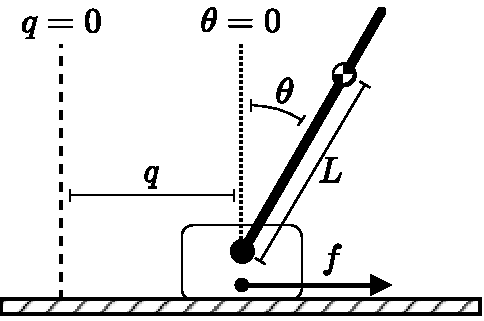
\includegraphics[width=0.4\textwidth]{assets/pic.png}
    \caption{Pic system. Qui ci va tutta la figura e la descrizione del sistema. }%todo
    \label{fig:pic}
\end{figure}




\section{Modello del sistema}
Nel paragrafo precedente ho detto che l'unica interazione possibile tra il sistema è l'esterno è l'applicazione di una forza sul carrello. Nella pratica, questo significa che è presente un motore vincolato al carrello in qualche modo. Mentre la natura del vincolo non è interessante, dobbiamo invece prestare particolare attenzione al tipo di motore utilizzato. Un motore esercita una forza che dipende sia da un segnale di controllo esterno, sia dallo stato interno dello stesso. È quindi conveniente separare lo studio del sistema in due: pendolo-carrello e motore.

\begin{figure}[thb]
    \centering
    %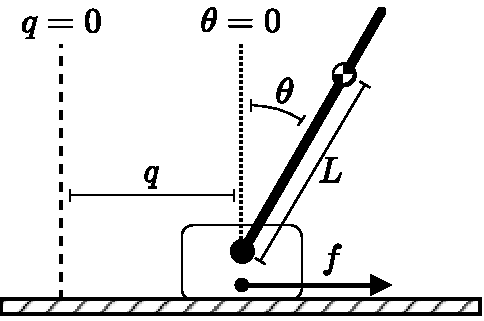
\includegraphics[width=0.4\textwidth]{assets/pic.png}
    \caption{Pic system. Qui ci va circa la stessa figura sopra, ma con l'immagine del motore collegato al carrello. }%todo
    \label{fig:pic-real}
\end{figure}

\subsection{Pendolo e carrello}
È immediato ricavare le equazioni del moto usando l'approccio Lagrangiano. Inizio fissando alcuni parametri che possono essere misurati sperimentalmente; sono riportati in tabella \ref{tab:parametri}. Posso quindi scrivere l'espressione per l'energia cinetica $T$ e potenziale $V$ del sistema:

\begin{equation*}
    \begin{aligned}
    T &= \frac 1 2 M  \dot x^2 +  \\ %todo
    V &= mgL \cos\theta
    \end{aligned}
    \hspace{20pt} \text{con } x \in \R, \theta \in ]-\pi, +\pi].
    \label{eq:energy}
\end{equation*}
La Lagrangiana $\mathcal L$ è data da:
\begin{equation*}
    \mathcal L = T - V
\end{equation*}
e posso ricavare le equazioni del moto usando le equazioni di Eulero:
\begin{equation*}
    \begin{aligned}
    asdasdasd %todo scrivi eq eulero
    \end{aligned}.
\end{equation*}
%todo
Qui ci dovrei mettere due considerazioni sulle forze (in particolare sugli attriti...)
Studio inoltre i punti di equilibrio del sistema:
\begin{equation*}
    \left. \frac \partial {\partial \theta}\right |_{V=V_{eq}} V =  0 \implies V_{eq} = \{0, \pi\}.
\end{equation*}


\begin{table}[htbp]
    \centering
    \begin{tabular}{@{}ll@{}}
        \toprule
        \textbf{Correct}     & \textbf{Incorrect}         \\
        \midrule
        \( A \implies B \)   & \( A \Rightarrow B \)      \\
        \( A \impliedby B \) & \( A \Leftarrow B \)       \\
        \( A \iff B \)       & \( A \Leftrightarrow B \)  \\
        \bottomrule
    \end{tabular}
    % Tra graffe ci sta il nome che viene visualizzato nell'elenco delle tabelle
    \caption[Parametri]{Parametri}
    %todo
    \label{tab:parametri}
\end{table}

\subsection{Motore}
\ref{https://homepages.laas.fr/lzaccari/seminars/DCmotors.pdf}
Per questa applicazione è sufficiente usare un motore DC brushless. Il motore è attivato applicando una differenza di potenziale tra le due armature e il verso di rotazione dipende dal segno della differenza di potenziale. Io voglio ricavare una relazione tra la coppia esercitata dal motore e la differenza di potenziale in ingresso.

Bla bla calcoli, modellino.
La stima dei parametri del motore la faccio sotto nella sezione "stima dei parametri del sistema".





\section{Linearizzazione e controllabilità}
vabb





\section{Strategia di swing-up}
Per lo swing-up, uso il metodo di Lyapunov così come descritto in [Astrom Furuta swinging up a pendulum by energy control]. 
%todo ref
Quello che voglio fare è:

\begin{enumerate}
    \item Studiare il moto del solo pendolo.
    %
    \item Trovare una funzione di Lyapunov per il solo pendolo.
    %
    \item Trovare una CLF per il solo pendolo.
    %
    \item Dalla CLF, ricavare una legge di controllo per lo swing-up.
\end{enumerate}
%todo glossary clf

\subsection{Energia del pendolo}
L'energia del solo pendolo è data da:
\begin{equation}
    E = T + V = \frac 1 2 I \dot \theta^2 + mgl(\cos\theta-1)
    \label{eq:energia-pendolo}
\end{equation}
dove ho scelto il potenziale in modo che si annulli quando $\theta=0$. Voglio studiare che effetto ha un accelerazione del polo $\Omega$ sul sistema. Posso farlo risolvendo l'equazione di eulero:
\begin{equation*}
    \frac {\partial^2} {\partial t \partial \dot \theta} \mathcal L - \frac \partial {\partial \theta} \mathcal L = -l ma \cos \theta 
\end{equation*}
dove compare la Lagrangiana $\mathcal L$ del solo pendolo e a secondo membro compare il momento torcente che l'accelerazione $a$ imprime al pendolo. Il risultato è che l'effetto dell'accelerazione $a$ del carrello sul pendolo è dato dall'equazione:
\begin{equation}
    I \ddot \theta - mgl\sin \theta + mal \cos \theta = 0
    \label{eq:moto-pendolo}
\end{equation}
\todo{qui ci starebbe bene un disegnino...}
%todo qui bisogna sistemare un po' i simboli
e posso usare le due equazioni \eqref{eq:moto-pendolo} e \eqref{eq:energia-pendolo} per calcolare la variazione di energia istantanea che produce l'accelerazione $a$ lungo la traiettoria del moto. Calcolo:
\begin{equation}
\begin{aligned}
    \partiald t E 
    &= \partiald t \left(\frac 1 2 I \dot \theta ^2 + mgl \cos \theta  \right) \\
    &= I \dot \theta \ddot \theta - mgl \sin \theta \cdot \dot \theta \\
    &= -mal \cos \theta \cdot \dot \theta
    .
    \label{eq:effetto-energia}
    \end{aligned}
\end{equation}
Già osservando la \eqref{eq:effetto-energia} posso ricavare una strategia di controllo rudimentale:
\begin{itemize}
    \item Se l'energia è minore di $0$, aggiungo energia al massimo rate possibile per il sistema: $a = a_{\text{max}}\sign{\dot \theta \cos \theta}$.
    \item Se l'energia è maggiore di $0$, tolgo energia al massimo rate possibile per il sistema: $a = -a_{\text{max}}\sign{\dot \theta \cos \theta}$.
\end{itemize}
Una strategia di questo tipo è detta \emph{bang-bang} e ha il vantaggio di essere la strategia che impiega mento tempo a raggiungere l'obiettivo, come conseguenza del principio di Pontryagins [qui devo vedere se spiegare primna il principio. Questa cosa comunque la spiega sempre Astrom in swing up with energy control...]. Tuttavia, una strategia di questo tipo è estremamente sensibile al rumore, in quanto piccole variazioni dell'energia creano discontinuità nel controllo.


\subsection{Funzione di Lyapunov e CLF}
Si può fare di meglio impiegando una CLF per ricavare una strategia di controllo. Questo permette sia di avere una strategia di controllo smooth, sia di dimostrare rigorosamente che il sistema raggiungerà l'equilibrio cercato, grazie ai teoremi ??\todo{qui dovrò citare teoremi scritti prima su controllabilità con lyapunov}. Inizio quindi definendo la funione di lyapunov \todo{dimostra che è una funzione di lyapunov?}:
\begin{equation}
    V = \frac 1 2 E^2.
    \label{eq:lyapunov-energy}
\end{equation}
Definire $V$ in questo modo mi permette di trovare una CLF molto semplicemente. Infatti, se calcolo la derivata rispetto al tempo lungo la traiettoria del moto...
\begin{equation}
    \partial t V = \frac 1 2 E^2.
    \label{eq:lyapunov-energy}
\end{equation}



\section{Stima dei parametri del sistema nel mondo reale}